% This paper is copyright 2021 the authors.

% people who might comment on it:
% -------------------------------
% - KSF
% - Kilian Walsh
% - Sanjoy Mahajan
% - David Grier

% style notes:
% ------------
% - Always air before water, always sail before keel before hull.
% - Need to choose typesetting for GoodSailing and BetterSailing and then be consistent.

% to-do items:
% ------------
% - FIND THE PRIOR LITERATURE!!
% - Overleaf seems to have wrong papersize?
% - Reconsider the post-equation commas? (HWR SAY).
% — Find references for, and destroy, Bernoulli.
% — Make some comments on the situations in which the ram-pressure force approximation is more appropriate---gale force or lull?
% - Is the latex footnote-footnote separation fucked?

\documentclass[letterpaper]{article}
\usepackage[utf8]{inputenc}
\usepackage{graphicx}
\graphicspath{{./}{../ipynb/}}
\usepackage{biblatex}
\addbibresource{sailing.bib}

% math macros
\usepackage{amsmath, amsfonts}
\DeclareMathOperator*{\argmax}{argmax}
\newcommand{\dd}{\mathrm{d}}
\renewcommand{\vec}[1]{\boldsymbol{#1}}
\newcommand{\uvec}{\vec{\hat{e}}}
\newcommand{\tensor}[1]{\mathbb{#1}}
\renewcommand{\flat}{\text{flat}}
\newcommand{\iso}{\text{iso}}
\newcommand{\air}{\text{air}}
\newcommand{\water}{\text{water}}
\newcommand{\boat}{\text{boat}}
\newcommand{\destination}{\text{dest}}
\newcommand{\good}{\text{(good)}}
\newcommand{\better}{\text{(better)}}
\newcommand{\sail}{\text{sail}}
\newcommand{\keel}{\text{keel}}
\newcommand{\hull}{\text{hull}}
\renewcommand{\above}{\text{above}}
\newcommand{\below}{\text{below}}
\newcommand{\vair}{\vec{v}_\air}
\newcommand{\vwater}{\vec{v}_\water}
\newcommand{\vboat}{\vec{v}_\boat}
\newcommand{\vdest}{\vec{v}_\destination}
\newcommand{\mps}{\mathrm{m\,s^{-1}}}

% text macros
\newcommand{\documentname}{\textsl{Article}}
\newcommand{\secref}[1]{Section~\ref{#1}}
\newcommand{\figref}[1]{Figure~\ref{#1}}

% typesetting adjustments
\makeatletter
\renewcommand\section{\@startsection {section}{1}{\z@}%
  {-3.25ex \@plus -1ex \@minus -.2ex}%
  {1.5ex \@plus .2ex}%
  {\raggedright\normalfont\large\bfseries}}
\makeatother
\setlength{\textwidth}{5.00in}
\setlength{\textheight}{9.00in}
\setlength{\topmargin}{-0.40in}
\pagestyle{myheadings}
\markright{\textsf{Hogg \& Kleban / Ram-pressure model for sailing}}
\newcommand{\figurerule}{\rule[1ex]{\textwidth}{0.2pt}}
\linespread{1.08}
\frenchspacing\sloppy\sloppypar\raggedbottom

\title{\bfseries%
A simple, anisotropic ram-pressure model for sailing}
\author{DWH, MK, others?}
\date{June 2021}
\begin{document}
\maketitle

\begin{abstract}\noindent
    We present a simplified model for the forces on a sailboat.
    Our model is that there is a ram-pressure force on the sail, with a magnitude and direction that depend on the alignment of the relative air--boat velocity with the sail orientation according to an anisotropic drag tensor.
    Similarly, there is a ram-pressure force on the keel, depending on the relative water--boat velocity.
    The resulting expression for the total force on the boat is coordinate-free and consistent with Galilean relativity.
    The solutions corresponding to sailing in steady wind correspond to boat velocities that deliver vanishing total force, given the angles of the sail and keel.
    We use this model to derive simple rules for sailing that are not far off from standard sailing practice, for sailing in different directions (including upwind).
    One consequence of this model is that a sailboat does not move (relative to the water) precisely in the direction that its keel points (the direction of the prow); it moves slightly downwind of that.
    Another consequence is that it is possible for an extremely anisotropic (extremely well designed) boat to sail downwind (relative to the water) \emph{faster than the wind}, on a tacking course.
    Interestingly, nothing about the mechanical model or discussion depend on the \emph{curvature} of the sail, in contradiction to some folk explanations of sailing.
\end{abstract}

\section{Introduction}\label{sec:intro}

HOGG: Why study sailing? What's the point?

KLEBAN: Write things about ddwfttw, maybe? For context only!

HOGG: Stuff about Bernoulli and flying and aerofoils that turned out to be wrong; a motivation to reconsider sailing too.

HOGG: What really is ram pressure? It is a model that the force comes mainly from momentum change or momentum transport in the fluid.

HOGG: Who is our audience? People interested in simple mechanics.
We eschew real fluid dynamics; we over-simplify.
This is possible because sailing is, in fact, very simple.

HOGG: We make use of good, coordinate-free expressions, a la \cite{kusse}.
We are Galilean-relativistic.

\section{Ram-pressure sailboat}\label{sec:boat}

We are going to work in 2D, with velocities $\vec{v}$ and forces $\vec{F}$ that are column vectors (or $2\times 1$ matrices).
To stay coordinate-free, we are going to talk about angles as orientations of unit vectors like $\uvec_{\perp\sail}$ and $\uvec_{\parallel\sail}$ (which will be defined below).
If you prefer to think in terms of angles, you can choose a coordinate system and then
\begin{align}
    \uvec_{\perp\sail} &= \begin{bmatrix}\cos\theta_\sail \\ \sin\theta_\sail\end{bmatrix} ~ ; ~ \uvec_{\parallel\sail} = \begin{bmatrix}-\sin\theta_\sail \\ \cos\theta_\sail\end{bmatrix} ~,
\end{align}
for some angle $\theta_\sail$ in that coordinate system.
We won't particularly use angles much in what follows, but if you want to come back to angles, you can take the arctangent of the components of $\uvec_{\perp\sail}$.

Our sailboat is going to be a simple anisotropic object such that wind that hits its planar sail produces a ram-pressure force perpendicular to the surface of the sail,
and water that hits its planar keel produces a ram-pressure force perpendicular to the surface of the keel.
We can construct the complete force law on the sailboat by thinking about ram-pressure forces on surfaces.
If the fluid (air or water in this case) is thought of as being composed of particles that bounce elastically off of a flat surface of area $A$, then the ram-pressure force on that surface is
\begin{align}\label{eq:flat}
    \vec{F}_\flat &= \eta\,\rho\,A\,(\uvec_\perp^\top\vec{v})^2\,\uvec_\perp ~,
\end{align}
where $\eta$ is a dimensionless prefactor, $\rho$ is the density of the fluid, $\uvec_\perp$ is the unit vector perpendicular to the surface (oriented such that it points down-flow), $\vec{v}$ is the velocity of the fluid in the rest frame of the surface, and $\uvec_\perp^\top\vec{v}$ is the scalar inner product (dot product) of the two vectors.
Na\"ively in the particle-collision model the prefactor $\eta$ is 2, but in the world of real fluids it depends on the shape of the surface, the velocity, and (if things are tiny) the viscosity\footnote{%
Viscosities only matter for very small objects, much smaller than sailboats. The way to see this is HOGG (CITE).}.
We're going to treat $\eta$ as an uninteresting constant; in particular we are going to assume that it doesn't depend on velocity, such that it can be combined with the area $A$ in everything that follows.
If you like thinking about tensors, the flat-surface force \eqref{eq:flat}  can be thought of as a tensor expression, in which $\rho$, $A$, and the unit vectors are combined into a three-index (order-three) tensor $\tensor{A}$, which is then contracted onto the velocity twice:
\begin{align}
    \tensor{A} &\equiv \eta\,A\,\uvec_\perp\,\uvec_\perp^\top\otimes\uvec_\perp^\top ~.
\end{align}
In Einstein summation notation, the three-index tensor is contracted as follows
\begin{align}
    [\vec{F}_\flat]_i &= \rho\,[\tensor{A}]_{ijk}\,[\vec{v}]_j\,[\vec{v}]_k ~,
    \\
    [\tensor{A}]_{ijk} &= \eta\,A\,[\uvec_\perp]_i\,[\uvec_\perp]_j\,[\uvec_\perp]_k
    ~,
\end{align}
where the $[\vec{v}]_i$ notation indicates the $i$th component or coordinate of the vector, the tensor $\tensor{A}$ has three indices, and the repeated indices are summed over.
If, instead of a planar object, you have an isotropic object (a sphere in fully 3D situations, an axi-symmetric boat in our 2D water world), the ram-pressure force becomes
\begin{align}\label{eq:iso}
    \vec{F}_\iso &= \eta\,\rho\,A\,|\vec{v}|\,\vec{v}
\end{align}
where $\eta$ is a (different) dimensionless prefactor, $A$ is now the cross-sectional or projected area of the surface, and $\vec{v}$ is still the fluid velocity in the rest frame of the object.
Again $\eta$ depends on velocity, but again we are going to ignore that.

Our model for a sailboat is going to be that it is a composite object, composed of a flat sail, a flat keel, and an isotropic partially submerged hull.
Thus the ram-pressure force on the sailboat will have four components, a force on the flat sail from the air, a force on the flat keel from the water, a force on the hull from the air, and a force on the hull from the water.
This model is extremely simplistic!
In some sense it is the closest possible model to the spherical cow that will sail non-trivially.
In detail the forces from the air are given by
\begin{align}\label{eq:startmodel}
  \vec{F}_\air &= \vec{F}_{\sail-\air} + \vec{F}_{\hull-\air}
  \\
  \vec{\Delta v}_\air &\equiv \vair - \vboat \label{eq:deltav}
  \\
  \vec{F}_{\sail-\air} & = \rho_\air\,A_\sail\,(\uvec_{\perp\sail}^\top\,\vec{\Delta v}_\air)^2\,\uvec_{\perp\sail} \label{eq:Fsailair}
  \\
  \vec{F}_{\hull-\air} & = \rho_\air\,A_{\above}\,|\vec{\Delta v}_\air|\,\vec{\Delta v}_\air ~,
\end{align}
where we have dropped the $\eta$ prefactors (or really combined them with the area constants), $\vair,\vboat$ are the velocities of the air and boat, $A_\sail$ is an area related to the area of the sail, $\uvec_{\perp\sail}$ is a unit vector perpendicular to the plane of the planar sail, and $A_{\above}$ is an area related to the area of the boat's hull that is above the water surface.
Similarly, the forces from the water are given by
\begin{align}
  \vec{F}_\water &= \vec{F}_{\keel-\water} + \vec{F}_{\hull-\water}
  \\
  \vec{\Delta v}_\water &\equiv \vwater - \vboat
  \\
  \vec{F}_{\keel-\water} & = \rho_\water\,A_\keel\,(\uvec_{\perp\keel}^\top\,\vec{\Delta v}_\water)^2\,\uvec_{\perp\keel}
  \\
  \vec{F}_{\hull-\water} & = \rho_\water\,A_{\below}\,|\vec{\Delta v}_\water|\,\vec{\Delta v}_\water ~,\label{eq:endmodel}
\end{align}
where the sail is replaced by the keel everywhere, and $A_{\below}$ is an area related to the area of the hull below the water surface.
HOGG NEED WE SAY MORE ABOUT THESE? PROBABLY YES THERE ARE COMMENTS TO BE MADE.

The above model could be called ``isotropic boat, thin planar sail and keel''.
There is an alternative model to be made, using the same elements, which could be called ``parallelepiped sail, parallelepiped keel''.
This alternative model uses only the flat-plane force law \eqref{eq:flat}, but the sail and keel each are treated as parallelepipeds with large areas $A_\sail$ and $A_\keel$ and then much smaller perpendicular areas $A_{\sail\parallel}$ and $A_{\keel\parallel}$.
So, for example, the force from the air on the boat in this model is
\begin{align}
  \vec{F}_\air &= \vec{F}_{\sail-\air} + \vec{F}_{\parallel-\air}
  \\
  \vec{F}_{\parallel-\air} & = \rho_\air\,A_{\sail\parallel}\,(\uvec_{\parallel\sail}^\top\,\vec{\Delta v}_\air)^2\,\uvec_{\parallel\sail}
   ~,
\end{align}
where $F_{\sail-\air}$ and $\vec{\Delta v}_\air$ are as defined in \eqref{eq:Fsailair} and \eqref{eq:deltav}, and $\uvec_{\parallel\sail}$ is the unit vector perpendicular to $\uvec_{\perp\sail}$.
The water force is similarly updated.
We have implemented both of these models, the isotropic boat with thin planar sail and keel, and the parallelepiped sail and parallelepiped keel.
Experimentation shows that these two models give almost exactly identical results, so choose whichever model you prefer.
In what follows, we use the \emph{isotropic boat with thin planar sail and keel} model of equations \eqref{eq:startmodel} through \eqref{eq:endmodel}.

\section{Steady sailing}\label{sec:steady}

Mathematically, steady sailing (constant $\vboat$) in steady wind and steady current (constant $\vair, \vwater$) is given by
\begin{align}\label{eq:sailing}
    \vec{F} &= \vec{F}_\air + \vec{F}_\water = \vec{0} ~.
\end{align}
If we want to operationalize steady sailing in code, steady sailing can be thought of as a root-finding problem, in which we find the vector $\vboat$ that makes \eqref{eq:sailing} true, given the orientations $\uvec_{\perp\sail}, \uvec_{\perp\keel}$ of the sail and keel.
This is a root-finding problem that (probably) has no closed form\footnote{%
It might be interesting to note that the flat-surface force \eqref{eq:flat} is a vector-valued quadratic form, so if one constructed the sailboat model completely from flat surfaces, the force law, in this approximation would be a quadratic form.
That might lead to a closed-form solution for the equation \eqref{eq:sailing} of steady sailing.}.
We solve equation~\eqref{eq:sailing} numerically in the code associated with this \documentname\footnote{%
HOGG GIVE LINK HERE}
by means of the vector generalization of Newton's method (we return to this in \secref{sec:implementation}).

HOGG: Define direction cosines with the wind, and with boat parts, using vectors. ADD THOSE direction cosines to the figure panels.

In \figref{fig:steady} we show examples of steady sailing, for a wide range of orientations of the keel and sail.
All these examples are shown in the water rest frame.
The boat has four free parameters $(A_\sail,A_\keel,A_{\above},A_{\below})$ all with units of area (or really three independent dimensionless ratios of these four areas).
The values we chose for these four parameters are given in \secref{sec:design} and discussed in detail there.
\begin{figure}[t!]
  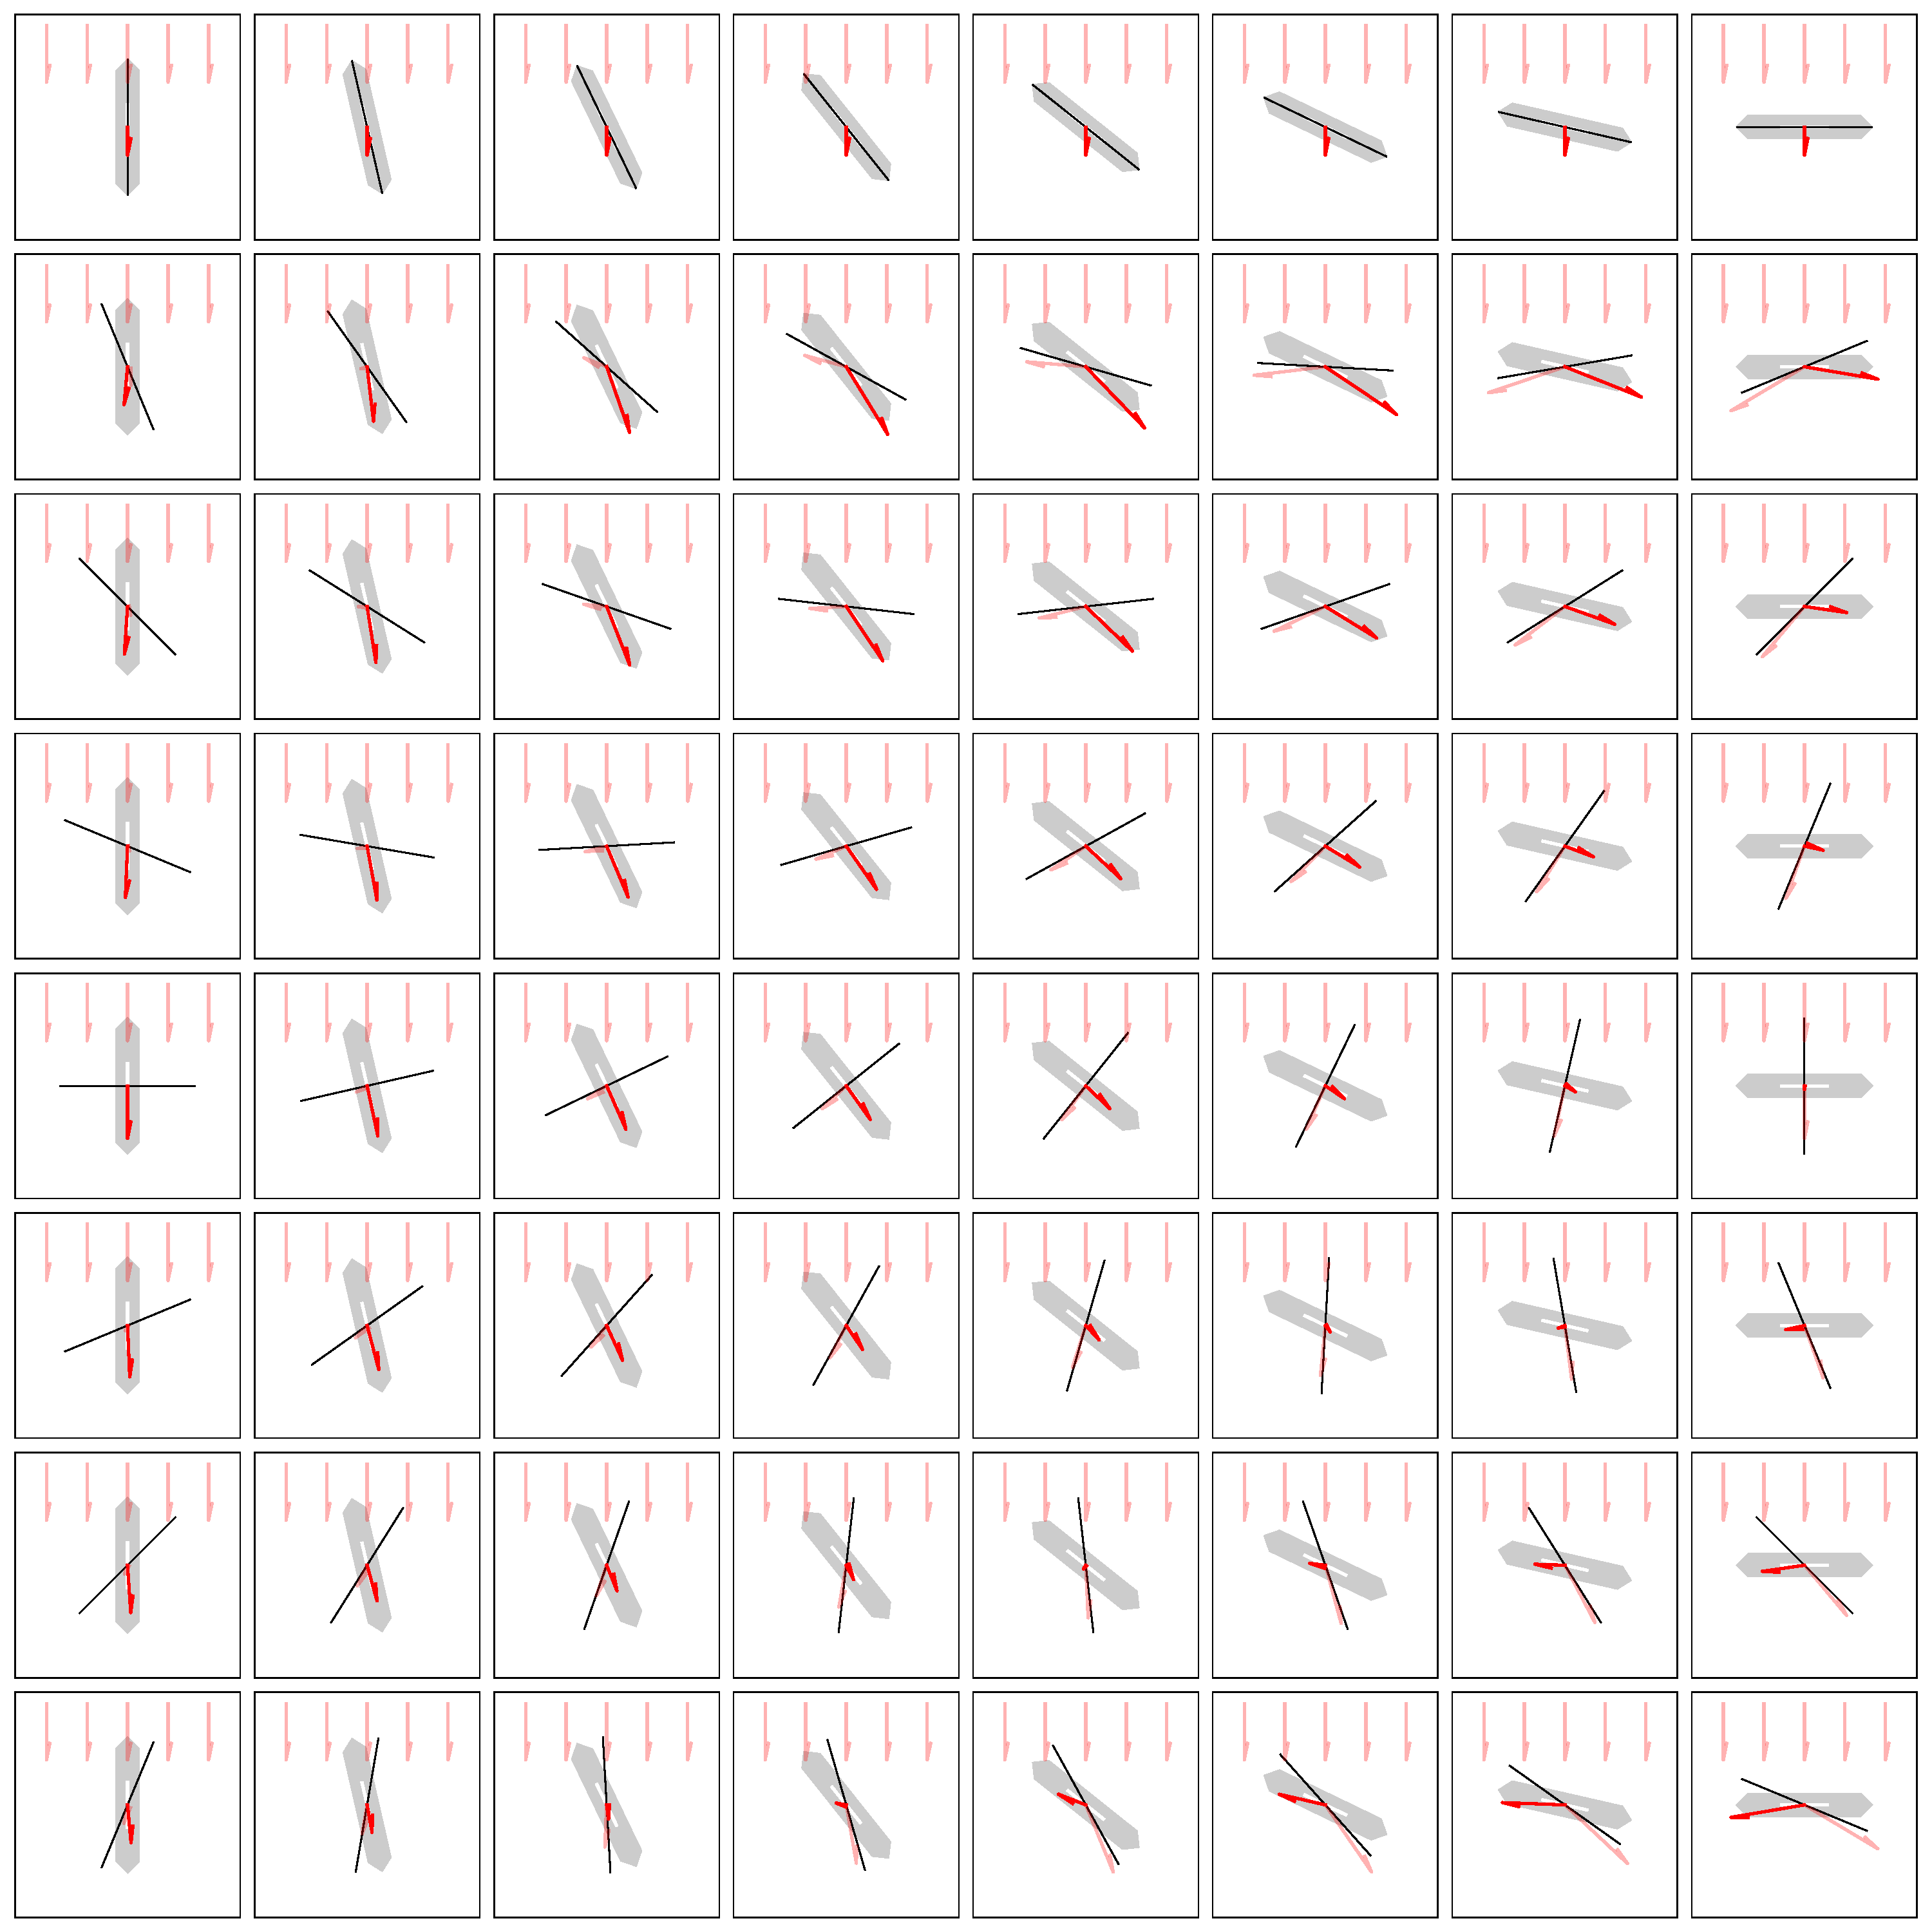
\includegraphics[width=\textwidth]{steady.pdf}
  \caption{Visualizations of the boat velocity $\vboat$ for different settings of the orientations of the keel and sail, all presented in the water rest frame.
  The views are top-down; the keel is represented by a thick grey line, the sail is represented by a thin black line, and the wind and boat velocities are represented by black arrows.
  Most of the settings of the keel and sail lead to downwind travel, but a few in the top-left quarter of this grid lead to upwind travel.\label{fig:steady}}
  \figurerule
\end{figure}

One comment to make is that if you look carefully at the panels of \figref{fig:steady}, you can see that, even in the rest frame of the water, the boat doesn't sail \emph{precisely} in the direction the keel is pointed.
It is close in most cases, but not precisely aligned.
This makes sense, because the wind is always---in some sense---trying to blow the sailboat downwind.

It might seem strange, in \figref{fig:steady}, that the keel orientation is marked but not the direction that the boat (the prow of the boat) is pointing.
Right now, the concept of ``forwards'' and ``backwards'' for the boat is a bit soft.
The boat is defined, in some sense, by the force laws.
These, in turn, are, in some sense, quadrupolar.
So the boat doesn't really have a front and a back!
We will get more serious about deliberately sailing in a particular direction in \secref{sec:good}.

In \figref{fig:hourglass} we show the distribution of relative boat--water velocities one obtains if one randomly orients one's sail and keel.
These orientations are literally randomly chosen angles from the uniform distribution on $[0,2\pi)$.
Many of the resulting boat--water velocities are near zero, because randomly orienting your keel and sail is not a good way to sail!
\begin{figure}[t!]
  ~\hfill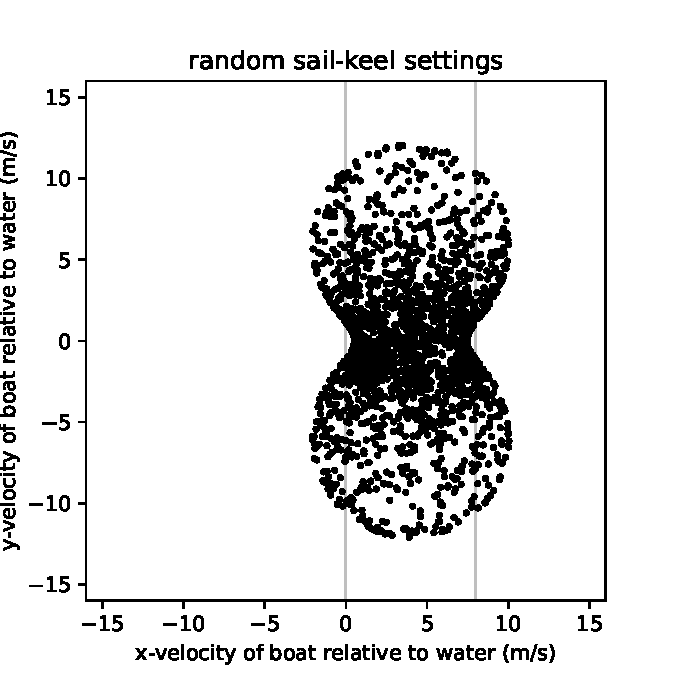
\includegraphics[width=3in]{hourglass-random.pdf}\hfill~
  \caption{The $x$ and $y$ coordinates of the relative boat--water velocity $\vboat-\vwater$ for a set of randomly oriented keels and sails.
  For all of these trials, the relative wind--water velocity is $\vair-\vwater=(8\,\mps)\,\uvec_x$ (that is, $8\,\mps$ in the $x$ direction), as it is in every panel of \figref{fig:steady}.
  Points to the left of the leftmost vertical grey line are sail--keel settings for which the boat sails upwind. Points to the right of the rightmost vertical grey line are sail--keel settings for which the boat sails downwind faster than the wind.
  There are no settings that go \emph{directly} upwind, and no settings that go \emph{directly} downwind faster than the wind.\label{fig:hourglass}}
  \figurerule
\end{figure}

There are many comments to make about the distribution of velocities shown in \figref{fig:hourglass}.
Here are a few:
There are many sail--keel settings that lead to travel at a boat--water velocity magnitude larger than the wind--water velocity magnitude.
You can't make any settings that give the boat precisely zero velocity with respect to the water.
The wind always blows it at least a bit.
There are many sail--keel settings that lead to downwind travel \emph{faster than the wind}.
Not \emph{directly} downwind faster than the wind, but faster than the wind.
That is, a sailboat can beat an air balloon at downwind travel even in stationary water!

There are, of course, many sail--keel settings that lead to upwind travel.
Not \emph{directly} upwind, but upwind.
That makes sense; the whole point (in some sense) of building a model of a sailboat is to understand how it sails upwind.
In \secref{sec:design} we will return to the upwind travel; we will show that in principle you might be able to build a boat that can travel upwind \emph{faster than the wind}.
Indeed, this boat (specs in \secref{sec:design}) does not sail upwind very fast, and it can't sail at an angle that is even close to directly upwind.
This closest angle to directly upwind will also be a function of the design of the boat.

One might ask: Intuitively, how does upwind travel work?
You can think of the boat like a slippery wedge, with the wind pushing on one side of the wedge (the sail) and the water pushing on the other side of the wedge (the keel).
The wedge slips forward.
Maybe that helps?

Finally, although upwind travel is slow going, with lots of tacking (HOGG DO WE NEED TO DEFINE THIS?) required, if you are situated \emph{on the boat}, upwind travel \emph{feels very fast}.
Why?
Because your experience of speed is, at least in part, the feeling of the wind in your face.
If you think about \figref{fig:hourglass} in terms of the boat-air velocity instead of the boat-water velocity---that is, if you Galilean-boost to the rest frame of the air---the upwind travel has much larger boat-air velocities than the downwind travel.
So even though you can sail fast downwind, it sometimes \emph{feels} faster upwind.

\section{Good sailing}\label{sec:good}

In \secref{sec:boat} we showed how the boat moves, given any arbitrary setting of the orientation of the keel and the sail.
However, one doesn't sail by randomly setting the keel and sail!
One sails by pointing the boat in some direction and then setting the sail (or sails) appropriately.
In our simple, ram-pressure boat, how should we set the planar sail?

HOGG: IN THIS SECTION EXPLICITLY DEFINE ``GOOD SAILING''.
\begin{align}\label{eq:good}
    \uvec_{\perp\sail}^\good &\leftarrow \argmax_{\uvec_{\perp\sail}} \left[\uvec_{\parallel\keel}^\top\,(\vboat-\vwater)\right] ~,
\end{align}
where .... HOGG IMPLICITLY $\vboat-\vwater$ is a function of all the properties of the world and the boat boat, along with the orientation of its keel and sail.

HOGG: FIGURE showing good sailing for a set of boat orientations.
\begin{figure}[t!]
  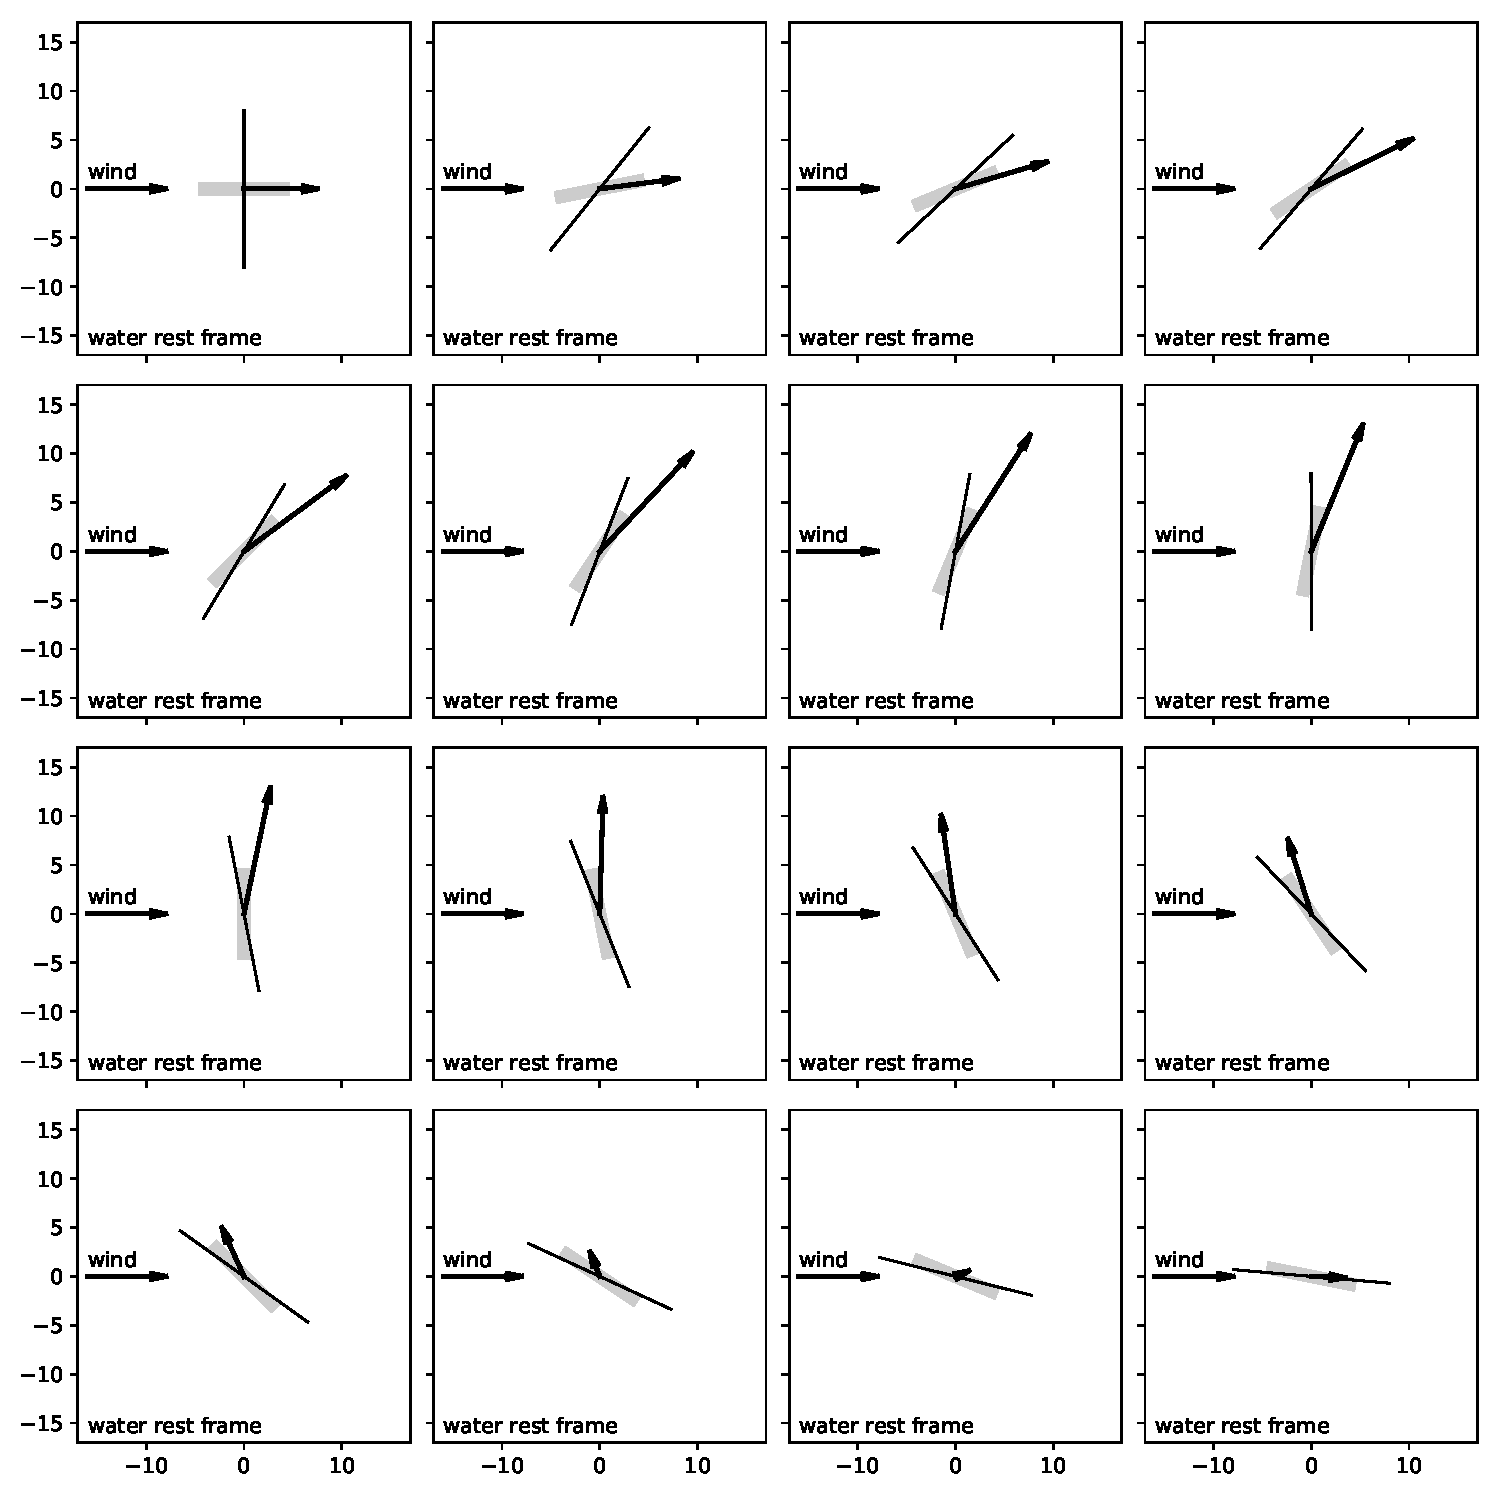
\includegraphics[width=\textwidth]{good.pdf}
  \caption{Visualizations of GoodSailing(tm) for different settings of the orientation of the keel.
  Conventions are the same as in \figref{fig:steady}.
  GoodSailing(tm) is unsuccessful in the last two cases, where the pointing is too close to directly upwind.
  In these cases the the maximum of the GoodSailing(tm) objective \eqref{eq:good} is negative.\label{fig:good}}
  \figurerule
\end{figure}

HOGG: Announce and discuss \figref{fig:hourgood}.
\begin{figure}[t!]
  ~\hfill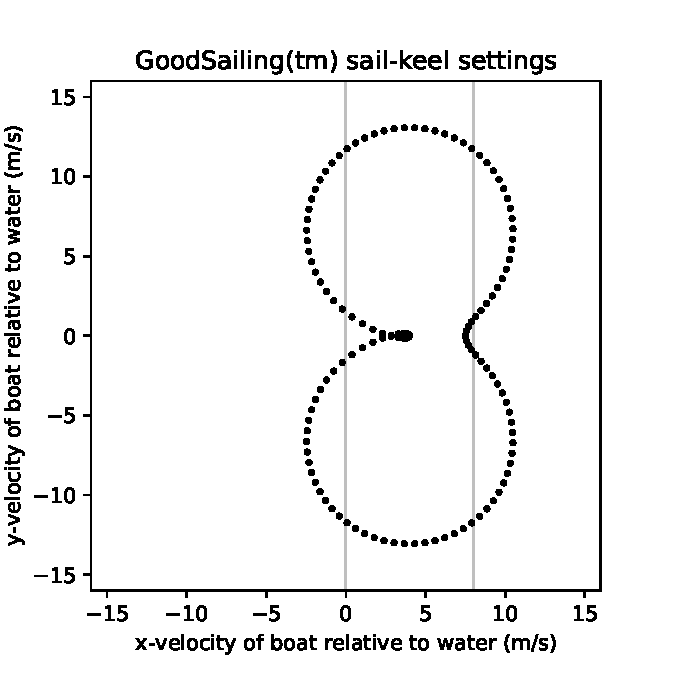
\includegraphics[width=3in]{hourglass-good.pdf}\hfill~
  \caption{The $x$ and $y$ coordinates of the relative boat--water velocity $\vboat-\vwater$ for GoodSailing(tm) for a set of randomly oriented keels.
  For all of these trials, the relative wind--water velocity is $\vair-\vwater=(8\,\mps)\,\uvec_x$ (that is, $8\,\mps$ in the $x$ direction), as it is in every panel of \figref{fig:good}.
  Compare this to \figref{fig:hourglass}.
  As is visible in \figref{fig:good}, when the keel orientation is too close to directly upwind, the boat goes downwind instead; there are no \emph{directly} upwind options.\label{fig:hourgood}}
  \figurerule
\end{figure}

HOGG: Figure showing direction cosines of sail relative to keel/boat orientation.

HOGG: Comment: The settings of the sail look ``tight'' relative to standard sailing practice. But this boat has flat sails, so it's hard to compare the exact settings with sailor experiences (which are all with curved sails).

HOGG: Final comment: But this is not the BEST a sailor can do...

\section{Better sailing}\label{sec:better}

HOGG IN THIS SECTION EXPLICITLY DEFINE ``BETTER SAILING''.

A type-A sailor---or maybe a competitive sailor---is trying to get from a current position to a destination as quickly as possible\footnote{%
We don't particularly endorse this attitude towards sailing. The journey \emph{is} the destination.}.
Our view is that this sailor should start by specifying the unit vector $\uvec_\destination$ that points from the current position of the boat towards the destination of the boat.
The sailor should then maximize the scalar product $\uvec_\destination^\top\,\vboat$
\begin{align}\label{eq:better}
    \uvec_{\perp\sail}^\better,\uvec_{\perp\keel}^\better &\leftarrow \argmax_{\uvec_{\perp\sail},\uvec_{\perp\keel}} \left[\uvec_\destination^\top\,(\vboat-\vdest)\right] ~,
\end{align}
where $\uvec_{\perp\sail}^\better,\uvec_{\perp\keel}^\better$ are the best settings of the orientations of the keel and sail, given the direction $\uvec_\destination$ to the destination, and (because we are Galilean-relativistic) this velocity is relative to the velocity $\vdest$ of the destination (which might not be stationary with respect to the water; imagine that we are sailing on a fast-flowing river).
In this expression \eqref{eq:better}, implicitly $\vboat$ is being thought of as a function of the orientations (and more).
Note that the sailor \emph{does not necessarily want} to travel directly towards the destination:
The sailor wants to make as much progress as possible in that direction, but is willing to tack back-and-forth to get there, if it gets the boat there faster.
So the optimization objective really is the projection of the boat velocity onto the displacement vector pointing from the current position of the boat to the destination.
While this is all simple to state, the global optimization is a bit painful to implement in code.
We give details in \secref{sec:implementation}.

HOGG PUT FIGURES HERE SHOWING THE OPTIMAL SETTINGS OF SAIL AND KEEL ORIENTATIONS FOR DIFFERENT DESTINATION DIRECTIONS.
\begin{figure}[t!]
  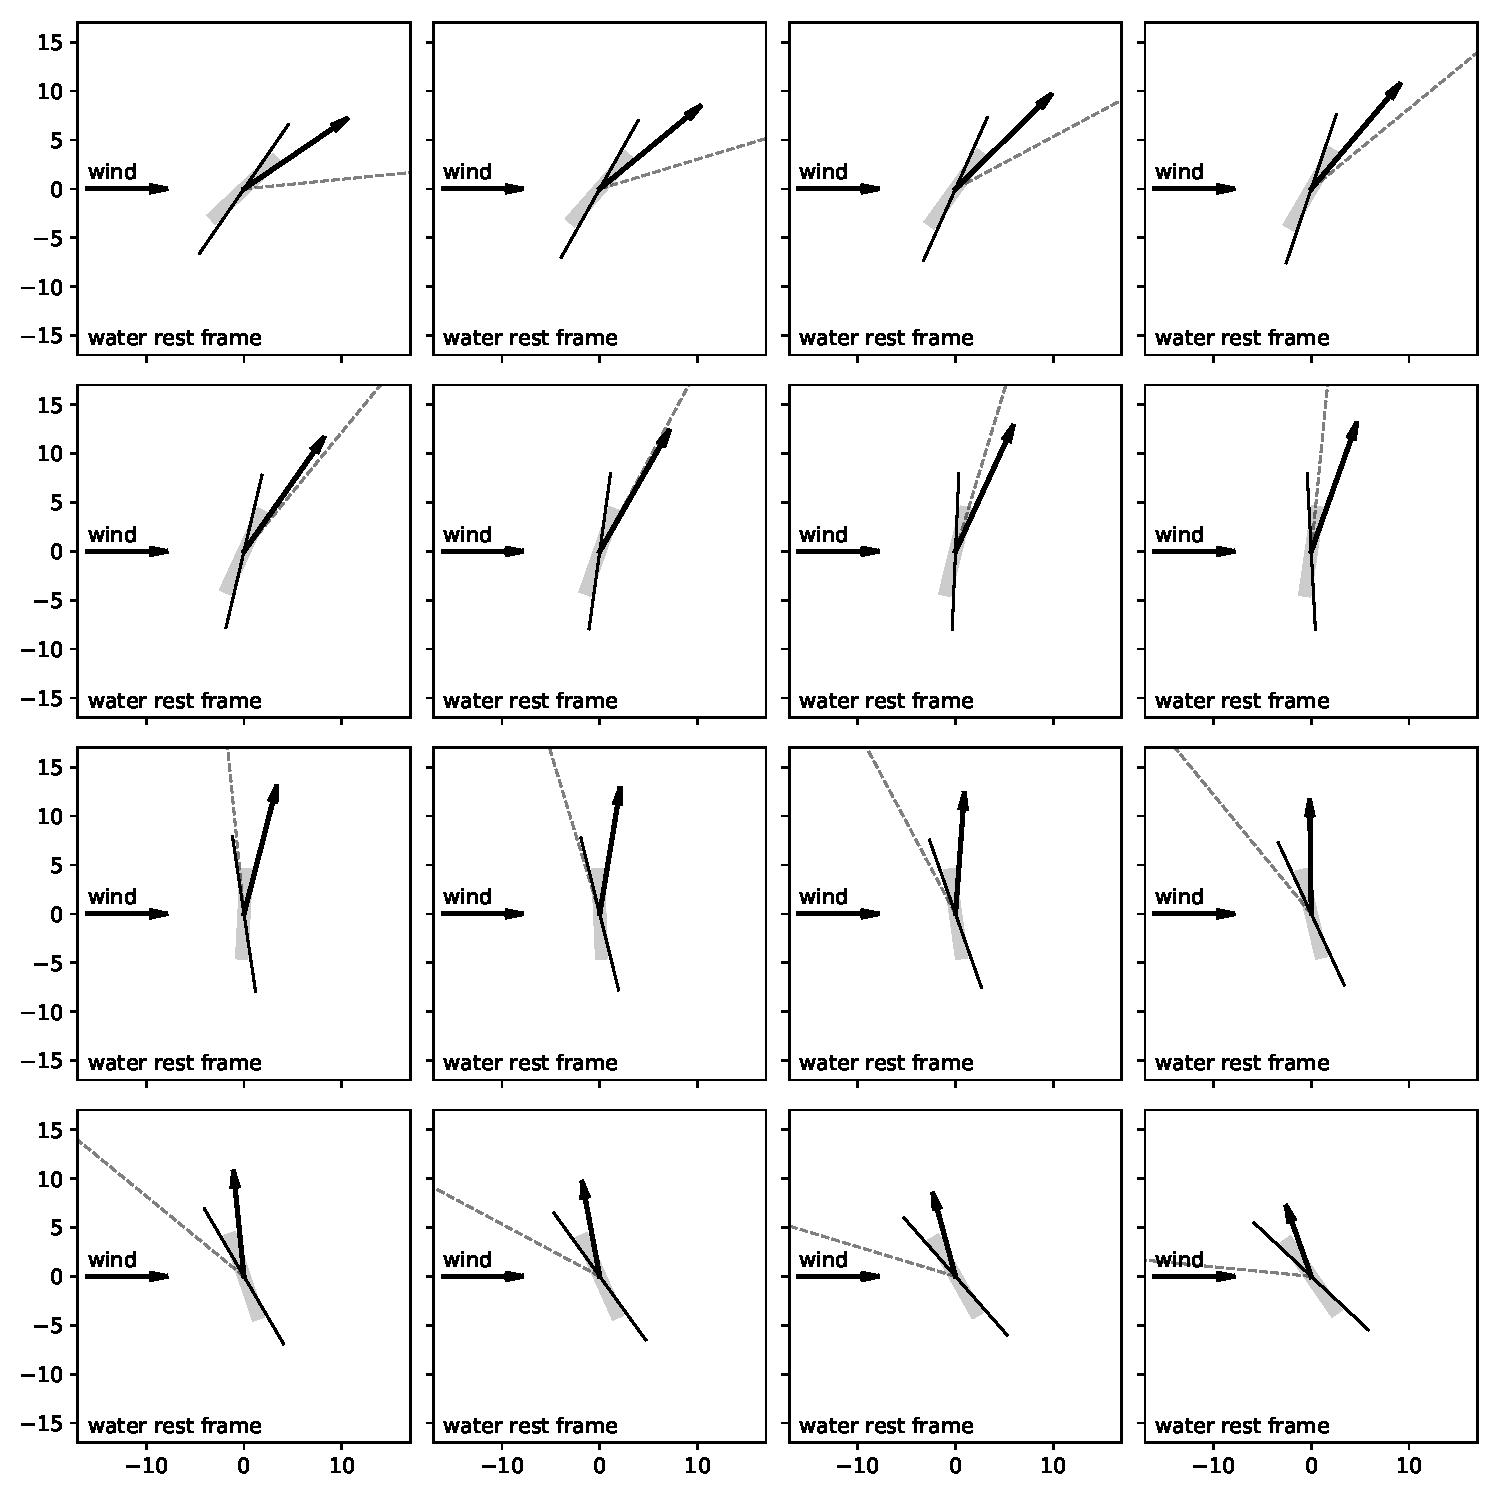
\includegraphics[width=\textwidth]{better.pdf}
  \caption{Visualizations of BetterSailing(tm) for different directions to a distant destination.
  Conventions are the same as in \figref{fig:steady} and \figref{fig:good}, except that now the destination direction is indicated with a dashed path line.
  These plots assume that the destination is stationary with respect to the water ($\vdest-\vwater=\vec{0}$).
  BetterSailing(tm) often involves sailing at a substantial angle to the direct line towards the destination.
  In these cases, the idea is that the best route to the destination involves frequent tacking back and forth across the path to the destination.\label{fig:better}}
  \figurerule
\end{figure}

HOGG discuss the hourglass figure.
\begin{figure}[t!]
  ~\hfill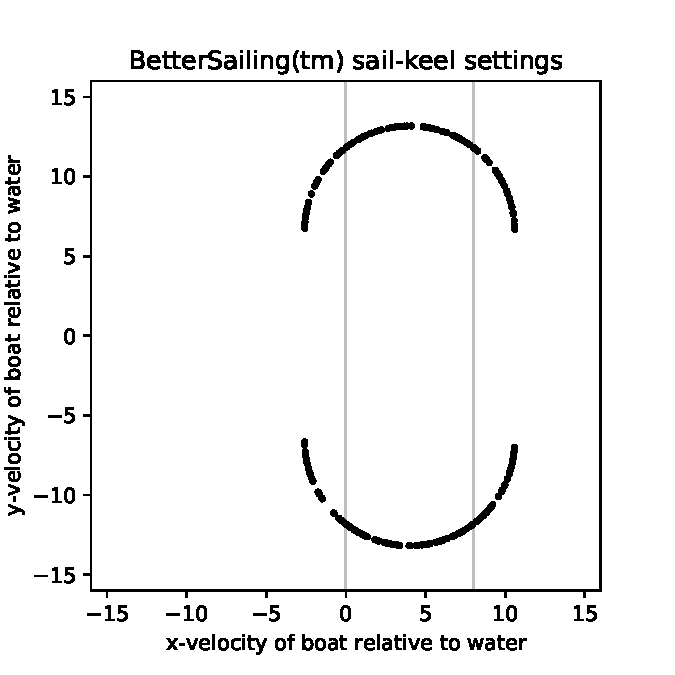
\includegraphics[width=3in]{hourglass-better.pdf}\hfill~
  \caption{The $x$ and $y$ coordinates of the relative boat--water velocity $\vboat-\vwater$ for BetterSailing(tm) for a set of randomly oriented destination vectors.
  For all of these trials, the relative wind--water velocity is $\vair-\vwater=(8\,\mps)\,\uvec_x$ (that is, $8\,\mps$ in the $x$ direction), as it is in every panel of \figref{fig:better}.
  Compare this to \figref{fig:hourglass} and also to \figref{fig:hourgood}.\label{fig:hourbetter}}
  \figurerule
\end{figure}

Now if you want to plan a complete path or journey for the sailboat in (unrealistically) steady wind, you... HOGG

HOGG PUT FIGURES HERE SHOWING TRAJECTORIES FOR SIMPLE JOURNEYS. MAYBE??

\section{Boat properties and boat design}\label{sec:design}

HOGG: In the above experiments and diagrams we made use of a boat with the following properties....

HOGG: These properties might seem unreasonable! However, remember that our boat is just a brutal approximation.
A true boat has sails that are globally curved\footnote{%
In the local-curvature or Riemann-curvature senses, sails are not (very) curved; after all, they are made from flat pieces of fabric.
However, they are curved in the global or colloquial sense: Different patches of the sail have differently oriented normal vectors.
It is in this colloquial sense that we are using the words ``curved'' and ``flat''.},
and forces that are different from these pure ram-pressure forces.
The curvature of the sails will in general rotate the air force vectors towards the direction in which the boat is pointed.

HOGG show how the hourglass plots depend on the qualities of the boat, such as: Relative area of sail and keel. Relative area of hull and keel. Etc.

\section{Numerical implementation notes}\label{sec:implementation}

HOGG: Newton's method (CITE), invert, solve, etc.
Note that in practice, Newton's method works amazingly well.
For Newton's method we make use of the derivatives---HOGG GIVE HERE THE DERIVATIVES of the ram-pressure expressions---which are order-2 tensors.

HOGG: How we implement GoodSailing(tm) and BetterSailing(tm) optimizations. It's a mess!

\section{Discussion}\label{sec:discussion}

HOGG: What did we find? What's important about that?

HOGG: Galilean symmetry, coordinate freedom?

HOGG: What were our assumptions? What are the myriad ways in which those assumptions must be wrong? For example, boat has an asymmetry in the wind too, so really the boat must also matter. Viscosity; why can we ignore it? But turbulence; we can't ignore that! Constant $\eta$ is also wrong.

HOGG: iso-planar vs parallelepipeds...

HOGG: Take some time to bash the Bernoulli bullshit.

HOGG: Even BetterSailing(tm) is not the best you can do, because you have to do complete successful path planning, and coming about costs time. So you will sail beyond the limits of BetterSailing(tm) if you do this correctly. This is out of scope for this \documentname.

HOGG: All code used to make the figures in this \documentname{} are available HOGG WHERE?

\paragraph{Acknowledgements:}
It is a pleasure to thank Hans-Walter Rix (MPIA) and Soledad Villar (JHU) for valuable discussions.

\raggedright
\printbibliography
\end{document}
